
\chapter[Hydrological conditions explain variation in wood density in riparian plants of south-eastern Australia][Wood density]{Hydrological conditions explain variation in wood density in riparian plants of south-eastern Australia}
\newpage

\section*{Abstract}
Wood density is a key plant functional trait which integrates the trade-offs characteristic to riparian plant ecological strategies. Although high density wood is costly to construct, it confers mechanical stiffness to stems, increasing a plant�s capacity to withstand flooding, and also enables increased tolerance to water stress. For riparian plants, fluctuations in soil moisture driven by surface hydrology should therefore be an important driver of variation in wood density.

We asked the following questions in the study: (1) does wood density increase with increasing frequency and magnitude of flood disturbance? (2) does wood density increase with increasing unpredictability of water availability in the riparian zone? (3) does dispersion of wood density peak at intermediate levels of hydrological disturbance?

We surveyed wood density of dominant species at 15 riparian sites along flow-gauged rivers across south-eastern Australia. Due to the broad range of hydrological variability associated with Australian river systems, this set of sites functions as a useful model for assessing the response of riparian plants to changing hydrological conditions. 

We found wood density varied strongly along a single axis of hydrological variability. This axis integrates flood intensity and frequency with metrics of hydrological unpredictability, and can be conceptualised as a gradient of environmental harshness, with higher wood density associated with harsher conditions. 

Our study highlights the importance of hydrological conditions, particularly disturbance and environmental unpredictability, as determinants of ecological strategy in riparian plants. Large, rare flood events in particular appear to favour higher wood density strategies. This is likely to have significant ecological consequences for riparian plant communities in a south-east Australian context, as well as in other regions where increasing climatic variability and frequency of extreme events are hallmarks of climate change predictions.

\clearpage

\section{Introduction}
Functional trait oriented approaches to understanding community assembly \citep{McGill2006} have become increasingly common over the last decade, particularly in the plant ecological literature \citep{Kattge2011}. These approaches attempt to understand community assembly processes by linking morphological or physiological attributes of species to organismal success under given environmental conditions. Suites of traits can be conceptualized as axes of variation in terms of �ecological strategy� and the distribution of this variation across environmental gradients can provide an insight into where these strategies are successful \citep{Westoby2002}.

Hydrology is widely considered to be the dominant abiotic force structuring riparian ecosystems \citep{Poff1997}. Hydrological variability in turn drives variation in moisture and substrate availability and flooding disturbance, with cyclical resets to early successional conditions being characteristic of the riparian environment \citep{Merritt2010}. These are the conditions which determine the dominant selection pressures and environmental filters, which in turn dictate success of a particular plant ecological strategy in a riparian system \citep{Naiman1997}. While ecohydrological classification is becoming established as a tool to explain plant community attributes such as species richness, stand structure and composition \citep{Poff2010a, Arthington2012}, to date only a small number of studies used functional approaches to investigating the ecohydrology of riparian plant communities \citep{bejarano2012, aguiar2013, stromberg2015riparian, Hough-Snee2015}, and use of quantitative functional traits has been rare.
  
Woody plants determine the coarse physical structure of many riparian plant communities and are integral to the interplay of biological and physical elements that drive fluvial biogeomorphic processes \citep{Corenblit2009}. Consequently, an understanding of the mechanisms of riparian woody plant community assembly will provide important insights into the structure and function of fluvial landscapes. Wood density, defined as the ratio of kiln-dried mass to green volume of a wood sample \citep{Cornelissen2003}, is widely recognised as an important functional trait in plant ecology \citep{Westoby2006, Swenson2007}, and has been proposed as one of just several key axes of variation within which all major plant ecological strategies can be described \citep{Westoby2002}. Wood density is in fact an emergent property of a combination of woody tissue traits, including vessel geometry and arrangement, and the density and proportion of surrounding lignified tissue \citep{Chave2009}. Combined variation in these traits corresponds to the wide range of wood density strategies among woody plants.
 
How might different wood density strategies confer advantages to woody plant species in riparian environments? There is little direct evidence from riparian species, however general relationships between wood density and other ecological traits have been recognised in a variety of different systems and can provide some insight into the importance of variation in wood density in riparian systems. Dense wood confers mechanical stiffness, but requires more investment of biomass and is therefore more costly to construct per unit of stem height \citep{Falster2006, Niklas2010}. Resources not invested in structural support may be used for purposes that contribute more directly to fitness, such as production of photosynthetic tissues or propagules, or rapid growth.

According to this trade-off, it follows that several relationships between wood density and life-history strategy are apparent. For example, wood density significantly explained variation in survival, fecundity and growth rate in a global dataset of 222 species \citep{Adler2014}. Studies of tropical rainforest species have shown an inverse relationship between growth rate and wood density \citep{King2006, Poorter2008, Poorter2010, Kraft2010, Wright2010}, although no such relationship was found in a study of New Zealand tree species \citep{Russo2010}. Cohort survival was positively correlated with wood density in the same tropical rainforest studies \citep{King2006, Poorter2008, Poorter2010, Kraft2010, Wright2010}. In a study of 45 rainforest species in tropical Queensland, \citep{Falster2005} found that wood density increased with plant height along a successional gradient. Following mechanical disturbance caused by a large cyclone in northern Queensland, Australia, wood density of rainforest trees was indicative of both damage sustained and subsequent recovery of biomass. Trees with dense wood were more likely to have experienced only minor damage. Of those trees that experienced major stem and branch damage, lower wood density trees were more likely to resprout and recover biomass faster post-disturbance \citep{Curran2008}. If the links observed in tropical rainforest communities between wood density, growth rate, successional status and recovery from mechanical disturbance hold true for riparian communities, the trade-off between rapid growth in response to high light and water availability, and construction of defences against flooding disturbance may be characteristic of woody plant ecological strategy in riparian zones.
  
In addition to influencing mean values of wood density, hydrological disturbance may also influence the dispersion of trait values within riparian communities. Niche diversity in riparian environments is promoted by fluvial geomorphic processes \citep{Corenblit2007}, and intermediate levels of disturbance have been theorised to promote divergence of disturbance-response strategies, resulting in a quadratic distribution of variance in associated trait values \citep{Grime2006, Sonnier2010}. 
While riparian plants potentially have the best access to water in a landscape, dramatic fluctuations in soil moisture are often characteristic of riparian environments \citep{Nilsson2002}. Ecological strategies for coping with unpredictable water availability may therefore be adaptive under these conditions. The relationship between wood density and precipitation-driven patterns of soil moisture is unclear. Some studies \citep{Weimann2002, Swenson2007} found little relationship between wood density and mean annual rainfall while others found that wood density was correlated with mean annual rainfall across a transcontinental gradient \citep{Martinez-Cabrera2009, Hacke2001, Larjavaara2010} and with soil moisture \citep{Preston2006}. High wood density, along with low specific leaf area (SLA) and low maximum height, has been linked  with environmental stress tolerance and conservative use of resources \citep{Westoby1998, Reich2003, Swenson2007}. Fluctuations in soil moisture driven primarily by hydrological conditions therefore should be an important driver of variation in wood density in riparian plant communities.
 
Given the extent to which flooding disturbance and fluctuations in water availability dominate riparian landscapes, woody tissue responses to these conditions are likely to be a primary indicator of riparian woody plant ecological strategy. Here we consider variation in wood density of dominant woody riparian plant species over a broad range of hydrological conditions, across 15 riparian sites within south-eastern Australia. As the most hydrologically variable continent on the planet \citep{finlayson1988australia, Peel2004}, Australia provides an ideal system to develop insight into the possible effects of increased hydrological variability in other regions under future climates. We sought to address the following questions:  (1) does wood density increase with increasing frequency and magnitude of flood disturbance? (2) does wood density increase with increasing unpredictability of water availability in the riparian zone? (3) does dispersion of wood density peak at intermediate levels of hydrological disturbance?

\section{Materials and methods}
\subsection{Study site selection}
Fifteen riparian sites were selected along gauged rivers within the South-East Coast and south-eastern Murray Darling drainage basins of Australia (Fig. \ref{fig:Ch2_F1}) (see Appendix 1 for further detail). To differentiate rivers according to ecologically relevant components of hydrology, \citep{Olden2003} described a statistical method for determining a minimally redundant set of hydrological descriptors. \citet{Kennard2010} followed this method to define a set of 120 hydrological metrics relevant to Australian rivers, which included metrics of central tendency and dispersion in all five dimensions of hydrological variation (magnitude, frequency, duration, timing, and rate of change) \citep{Kennard2010}. These metrics were then used to classify Australian river systems into twelve distinct flow regime classes, providing a foundation for analysing the properties of ecosystems across hydrological gradients. In this study, sites were drawn from rivers corresponding to �stable winter baseflow�, �unpredictable baseflow� and �unpredictable intermittent� hydrological classes, as described by Kennard et al (2010). These are the best represented hydrological classes in eastern New South Wales and Victoria, and combined, span clear gradients of flooding intensity and hydrological unpredictability. 

Five sites per hydrological class were selected based on the following criteria: gauged locations were selected that had $>$15 years of associated continuous hydrological data, and an absence of flow regulation, significant water extraction or catchment urbanisation, following \citet{Kennard2010}. To minimise signals associated with human land-use and river type, the following further criteria were used to shortlist possible study sites: all were partly confined valleys with discontinuous floodplain pocket River Styles, \textit{c.f.} Brierley \& Fryirs (2005) \citep{brierley2008geomorphology}, had an intact native riparian vegetation cover (a band of native riparian vegetation extending $>$15 m from the bankfull channel edge), were in good geomorphic condition (lack of significant human-induced erosional or depositional landforms), minimal vegetation clearing (catchment predominantly covered by native vegetation) and occurred in a catchment smaller than 1000 km\textsuperscript{2}. These criteria were assessed using a combination of visual inspection of satellite photography (Google Earth, Microsoft Bing) and information from the NSW Riparian Vegetation Extent dataset and the NSW Office of Water River Styles� geospatial dataset \citep{Healy2012}. To select the 15 study sites from this shortlist, accessibility by road, permission from state or private landholders, and proximity of accessible areas to continuous hydrological monitoring stations were taken into account.

%%%% FIGURE 1
\begin{figure}[ht]
\begin{center}
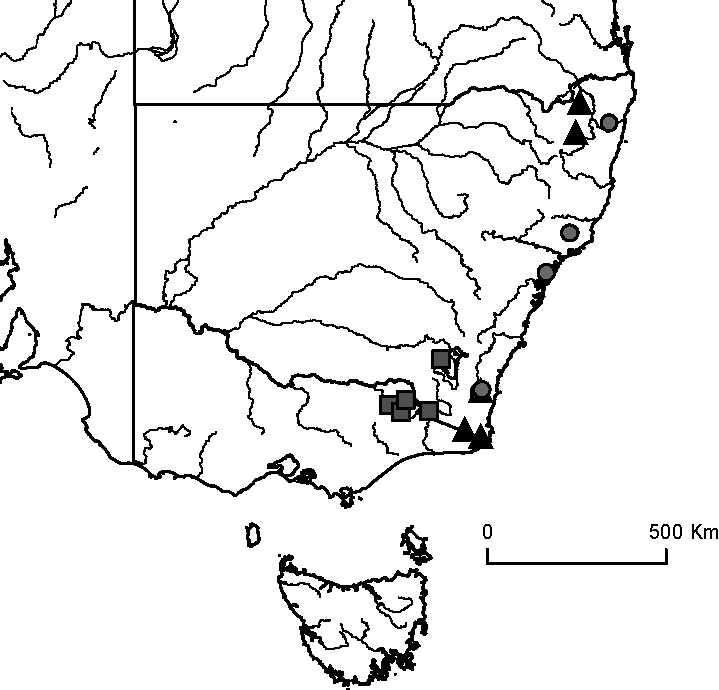
\includegraphics[width=12cm,keepaspectratio=true]{Ch2map.pdf} % figures can be in pdf, png, jpeg or eps format
\caption[Location of fifteen field study sites across south-eastern Australia.]{\small{Location of fifteen field study sites across south-eastern Australia chosen to represent the three major hydrological classes of south-east Australia. Hydrological class membership is denoted by:  $\blacksquare$ stable winter baseflow, $\blacktriangle$ unpredictable baseflow, \textbullet  unpredictable intermittent.}}
\label{fig:Ch2_F1} % label for cross-referencing
\end{center}
\end{figure}   
\clearpage

\subsection{Species abundance and trait data collection}
Data collection was undertaken between December 2012 and May 2013. At each site, a 10 m by 50 m plot was marked out, with the longest edge abutting the channel edge. Criteria for selection of plot locations were: geomorphic homogeneity (the plot comprising only sloping bank where possible) and lack of anthropogenic disturbance such as built structures, roads or tracks, recent logging or clearing (in the last 20-30 years), herbicide spraying or animal grazing. Variation in the maximum height above the channel edge between plots was kept to within approximately 1.5 m.

Proportional cover of all woody species was assessed within three strata: shrub (1-4 m), sub canopy (4-8 m) and canopy ($>$8 m). Species were identified using appropriate field guides, and were verified against herbarium specimens at the Macquarie University Herbarium. Some specimens were identified by staff at the Royal Botanic Gardens, Sydney. 

Wood samples were collected from woody species present within the plot at $>$1\% cover in shrub, sub canopy or canopy strata, and which had trunks robust enough to core. A 100 mm wood sample from each of two individuals per species was extracted using a 5.15 mm diameter, triple threaded increment borer (Hagl�f Sweden). Samples were extracted from the base of the main trunk, 10 cm above the leaf litter level, and air-dried at 20-45 \textsuperscript{o}C. On return to the laboratory, samples were rehydrated to saturation in deionised water and 10 mm sections of mature heartwood were cut flush with a razor, using visual inspection of vessel occlusion as an indicator of maturity. Sections were measured (x, y and z dimensions) to the nearest 0.01 mm with callipers (Mitutoyo America, Illinois USA) to calculate wet volume, then oven-dried at 80 \textsuperscript{o}C for 48 hours and weighed using a microbalance (Mettler Toledo, Greifensee, Switzerland). Wood density was then calculated as the ratio of oven dry mass to wet volume (g/cm\textsuperscript{3}).

Species which were present in plots but which could not be cored due to small size were assigned averaged values of wood density from the same species measured at other sites, where possible. Remaining species were assigned values from peer-reviewed literature sources. Appendix 1a contains further details about the dataset, including data density information.

\subsection{Hydrological analysis}
Daily discharge data pertaining to each field site were collated from the PINNENA CW 10.1 database (NSW Office of Water, Department of Primary Industries) and the NSW Office of Water Continuous Water Monitoring network website \url{(http://realtimedata.water.nsw.gov.au/water.stm)} for NSW sites, and the Victoria State Government�s Water Measurement Information System website \url{(http://data.water.vic.gov.au/monitoring.htm)} for Victorian sites. Where possible, 30 year time series were obtained, spanning years 1983 � 2012. Records were truncated for three sites, spanning 15, 19 and 28 years. Missing data were approximated using the Time Series Manager module in River Analysis Package \citep{marsh2003river}. Consistency of the resulting outputs were checked by visual inspection of hydrographs. For Mammy Johnson�s River, Mann River, Sportsman�s Creek and Wallagaraugh River, multiple linear regression was chosen as the most appropriate method for estimating missing data values. Linear interpolation was used for Jilliby Creek data. Daily discharge data for the remaining sites were complete.

A set of 24 hydrological metrics was pared from the full set described by \citet{Kennard2010}.  These metrics were chosen to be representative of variability in high flow magnitude and frequency as well as predictability and consistency of water availability in the riparian environment (see Table \ref{tab:Ch2_T1} for a description). We used the Time Series Analysis module in River Analysis Package to generate these metrics. Means and coefficients of variation were calculated for most metrics to indicate central tendency as well as spread within the data. Low and high spell metrics were thresholded at the 5th and 95th percentiles, respectively, with a flood independence criterion of 7 days between peak events. Twenty year average return interval (ARI) flood magnitude was also calculated with a flood independence value of 7 days between peaks. Colwell's Indices were calculated using mean flow values over monthly time periods and a class distribution of 11 flow classes. Metrics of flow magnitude which had units ML / day were normalised by mean daily flow to allow for comparison between different sizes of river. Some metrics were correlated (see Appendix 1a for correlation analysis).


\begin{landscape}
\begin{tiny}
{\tabulinesep=1.2mm
\begin{longtabu} to \linewidth {m{5.5cm}m{3.7cm}m{2.0cm}X} 
\caption[Description of hydrological variables.]{Hydrological parameters used as metrics of variability in high flow magnitude and frequency and predictability and consistency of water availability in the riparian environment. * - normalised by mean daily flow (ML/day)} \\
\label{tab:Ch2_T1} \\
\hline
% -----------------These are headings----------------------------------%
\textit{Variable} & \textit{Abbreviation} & \textit{Units} & \textit{Description} \\ 
%
\endfirsthead
%
%\multicolumn{4}{c}%
%{{\bfseries  Continued from previous page}} \\
%\hline
%
\hline
\textit{Variable} & \textit{Abbreviation} & \textit{Units} & \textit{Description} \\ \hline
\endhead
%
%\hline \multicolumn{4}{|r|}{{Continued on next page}} \\ \hline
%\endfoot
%
%\hline
%\multicolumn{4}{|r|}{{Concluded}} \\ \hline
%-----------Headings end---------------------------------
%\endlastfoot
\hline
\multicolumn{4}{l}{\textbf{Flood frequency and magnitude}} \\
Mean magnitude of high spells * & HSPeak & dimensionless & \multirow{1}{*}{\parbox{8.2cm}{High spells are periods of flow above the 95th percentile on the flow duration curve. We were interested in how frequently these conditions occurred over the time series as well as the mean magnitude of peak flows during these periods. 20 year average return interval (ARI) floods are extreme flow events that have the potential to re-work the fluvial landscape. Together, these metrics indicate the intensity and frequency of mechanical stress experienced by plants in the riparian zone.}} \\
CV of all years' mean high spell magnitude & CVAnnHSPeak & dimensionless &  \\
20 year ARI flood magnitude * & AS20YrARI & dimensionless &  \\
Mean of all years' number of high spells & MDFAnnHSNum & year\textsuperscript{-1} &  \\
CV of all years' number of high spells & CVAnnHSNum & dimensionless &  \\[0.6cm]
%\tabularnewline
\hline
\multicolumn{4}{l}{\textbf{Rise and fall rates}} \\
Mean rate of rise * & MRateRise & day\textsuperscript{-1} & \multirow{1}{*}{\parbox{8.2cm}{Rise and fall rates represent flow �flashiness�. Fast rise rates are associated with flood waves and intense mechanical stress to plant stems. Slow fall rates keep exposed substrate moist for longer periods, which may produce favourable conditions for germination. Historical discharge records are unfortunately limited to daily resolution, so are unable to fully capture flood discharge shapes. High variability between years indicates the occurrence of extreme events which may not have been captured by the mean value.}} \\
Mean rate of fall * & MRateFall & day\textsuperscript{-1} &  \\
CV of all years' mean rate of rise & CVAnnMRateRise & dimensionless &  \\
CV of all years' mean rate of fall & CVAnnMRateFall & dimensionless &  \\[1.1cm] 
%\tabularnewline
%\tabularnewline
\hline
\newpage
\multicolumn{4}{l}{\textbf{Baseflow index}} \\
Baseflow index & BFI & dimensionless & \multirow{1}{*}{\parbox{8.2cm}{Baseflow index is calculated using the ratio of flow during average conditions to total flow. It is a useful metric of consistency of water availability, in that it is maximised when average flow conditions dominate, and minimised when total flow is dominated by above average flow events. Intra-annual variability in baseflow index measures how predictable baseflow index is between years.}} \\
CV of all years' Baseflow Index & CVAnnBFI & dimensionless &  \\[1.2cm]
%& & & & \\
%\tabularnewline
\hline
\multicolumn{4}{l}{\textbf{Low flow magnitude, frequency and duration}} \\
CV of all years' mean low spell magnitude & LSPeak & dimensionless & \multirow{1}{*}{\parbox{8.2cm}{Low spells are periods of flow below the 5th percentile on the flow duration curve. We were interested in how frequently these conditions occurred over the time series as well as the mean and interannual variability in magnitude and duration of low flows.}} \\
Mean magnitude of low spells & CVAnnLSPeak & dimensionless &  \\
Mean of all years' number of low spells & MDFAnnLSNum & year\textsuperscript{-1} &  \\
CV of all years' number of low spells & CVAnnLSNum & dimensionless &  \\
Mean duration of low spells & LSMeanDur & days &  \\
CV of all years' low spell mean duration & CVAnnLSMeanDur & dimensionless &  \\
Mean flow during driest week of the year * & MA.7daysMinMean & dimensionless &  \\
Mean days per year under 0.1ML/day flow & MDFAnnUnder0.1 & days/year &  \\
CV of all years' days per year under 0.1ML/day flow & CVAnnMDFAnnUnder0.1 & dimensionless &  \\[0.3cm]
%\tabularnewline
\hline
\newpage
\multicolumn{4}{l}{\textbf{Colwell's indices}} \\
Constancy of monthly mean daily flow & C\_MDFM & dimensionless & \multirow{1}{*}{\parbox{8.2cm}{Colwell's indices provide a measure of the seasonal predictability of flow events and therefore water availability within the riparian zone. Constancy (C) measures uniformity of flow across seasons, and is maximised when flow conditions do not differ between seasons. Contingency (M) is a measure of interannual uniformity in seasonal flow patterns, and is maximized when seasonal patterns of flow are consistent between years.  We generated Colwell's indices for both average flow conditions and minimum flows conditions.}} \\
Contingency of monthly mean daily flow & M\_MDFM & dimensionless &  \\
Constancy based on monthly minimum daily flow & C\_MinM & dimensionless &  \\
Contingency based on monthly minimum daily flow & M\_MinM & dimensionless & \\[0.9cm]
%\tabularnewline
\hline
\end{longtabu}}
\end{tiny}
\end{landscape}
\clearpage

\subsection{Wood density analysis}
All statistical analyses were performed using the R statistical programming environment \citep{RCoreTeam2015}. The R code used for these analyses can be retrieved from \url{https://github.com/jamesrlawson/riparian-WD/tree/master/scripts}. Statistical significance was interpreted at alpha = 0.05. 

\subsubsection{Characterising community-level variation in wood density}
To investigate variation in wood density across hydrological gradients at the community level, community weighted means (CWM) of wood density were generated for each site. Species relative abundance was compiled from records of percent cover at the shrub (1-4 m), sub canopy (4-8 m) and canopy ($>$8 m) strata.  Wood density values were then weighted according to species relative abundance and summed to produce the CWM. This method integrates particular trait values with their real world abundance as a measure of �performance�, while providing a useful reduction in data dimensionality. Wood density varies only over one order of magnitude, while exhibiting relatively high intra-species plasticity. As such, CWMs work well for environmental gradient studies of wood density because the focus is maintained on the functional characteristics of the community, rather than on species \textit{per se}.

We also calculated community weighted variance (CWV) in wood density for each site to characterise the dispersion of wood density values within communities. CWV describes divergence from the mean trait value of a community \citep{Schleuter2010}. When trait values of abundant species are clustered towards the mean, divergence is low. Conversely, divergence is high when abundant species are distributed towards the extremes of the trait range \citep{Villeger2008}. Variance could not be calculated for Site 2 (Wallagaraugh River, unpredictable baseflow category) as only a single woody species was found at $>$ 1 \% cover at this site. This site was therefore omitted from subsequent analyses of CWV.

\subsubsection{Testing relationships between wood density and hydrological conditions}
Ordinary least-squares regression models were generated for selected metrics to determine relationships between hydrological gradients and CWMs. Linear models were used except where non-linear relationships were obvious. Wood density data was normally distributed and did not require transformation. To reduce the occurrence of Type 1 statistical error, we adjusted the resulting p values using the Benjamini - Hochberg (BH) procedure for controlling family-wise error rate (stats package) \citep{RCoreTeam2015}. Although ecological rationale supported inclusion of each subgroup of hydrological metrics, a number of these metrics were correlated. The BH procedure has been shown to control the false discovery rate for positively dependent test statistics \citep{Benjamini2001}.

We identified ecologically relevant axes of variation in hydrological conditions by running a principal components analysis (stats package), \citep{RCoreTeam2015} for hydrological metrics which had significant relationships with site mean wood density values. Having established the dominance of a single relevant axis of variation in hydrology (refer Fig. \ref{fig:Ch2_F5}), we tested the fit of a quadratic model relating extent of hydrological disturbance (as characterised by site scores from the resulting first principal component) to CWV in wood density.

Spatial autocorrelation in CWM and CWV values was assessed using Moran's I (ape package), \citep{Paradis2004}.

\section{Results}
\subsection{How does mean wood density change over hydrological gradients?}
Below we describe patterns of community weighted mean wood density in relation to the hydrological variables divided into two groups: those describing frequency and magnitude of flood disturbance, and those describing predictability of water availability in the riparian zone. Regression statistics for all models are given in Table \ref{tab:Ch2_T2}.

Community mean wood density varied by 50 \% between sites. The largest, most intense flood events throughout a river�s hydrological record were found to show a strong positive relationships with mean wood density (Fig. \ref{fig:Ch2_F2}a, \ref{fig:Ch2_F2}b. Flooding frequency had no influence on wood density. Mean flood rise rate (Fig. \ref{fig:Ch2_F2}c) as well as interannual variability in flood rise and fall rates (Fig. \ref{fig:Ch2_F2}d, \ref{fig:Ch2_F2}e) were positively related to wood density; this relationship was considerably stronger for interannual variability in flood rise rate than mean flood rise rate (R2 = 0.549 vs 0.360).

\begin{table}[ht]
\doublespacing
\tiny
\centering
\caption[Statistics for regression models.]{\small{Statistics for regression models comparing hydrological metrics with site mean wood density. P.adj denotes p values adjusted by the Benjamini-Hochberg method. Significant results are shown in bold. Models used are either quadratic or linear, as shown in Fig. \ref{fig:Ch2_F2} and Fig. \ref{fig:Ch2_F3}. For non-significant relationships, statistics shown are for linear models.}}
\label{tab:Ch2_T2}
{\tabulinesep=1.2mm
\begin{tabu}to \textwidth {XXXX}
\hline
\textit{Variable}          & \textit{P}     & \textit{P.adj} & \textit{R\textsuperscript{2}}    \\ \hline
CVAnnBFI        & 0.008 & 0.031 & 0.549 \\
CVAnnMRateRise  & 0.008 & 0.031 & 0.549 \\
C\_MinM         & 0.009 & 0.031 & 0.542 \\
C\_MDFM         & 0.012 & 0.031 & 0.522 \\
HSPeak          & 0.004 & 0.031 & 0.485 \\
AS20YrARI       & 0.005 & 0.031 & 0.467 \\
LSPeak          & 0.006 & 0.031 & 0.447 \\
CVAnnMRateFall  & 0.007 & 0.031 & 0.435 \\
BFI             & 0.012 & 0.031 & 0.397 \\
M\_MDFM         & 0.013 & 0.031 & 0.388 \\
MA.7daysMinMean & 0.017 & 0.036 & 0.368 \\
MRateRise       & 0.018 & 0.036 & 0.360 \\
MDFAnnLSNum     & 0.030 & 0.055 & 0.314 \\
MRateFall       & 0.053 & 0.091 & 0.258 \\
M\_MinM         & 0.062 & 0.100 & 0.242 \\
CVAnnHSPeak     & 0.117 & 0.175 & 0.178 \\
LSMeanDur       & 0.230 & 0.325 & 0.109 \\
CVAnnLSPeak     & 0.390 & 0.493 & 0.057 \\
CVAnnHSNum      & 0.390 & 0.493 & 0.057 \\
CVAnnLSNum      & 0.454 & 0.545 & 0.044 \\
MDFAnnUnder0.1  & 0.487 & 0.556 & 0.038 \\
MDFAnnZer       & 0.553 & 0.603 & 0.028 \\
CVAnnLSMeanDur  & 0.732 & 0.747 & 0.009 \\
MDFAnnHSNum     & 0.747 & 0.747 & 0.008 \\[0.1cm] \hline
\end{tabu}}
\end{table}

%%%% FIGURE 2
\begin{figure}[ht]
\begin{center}
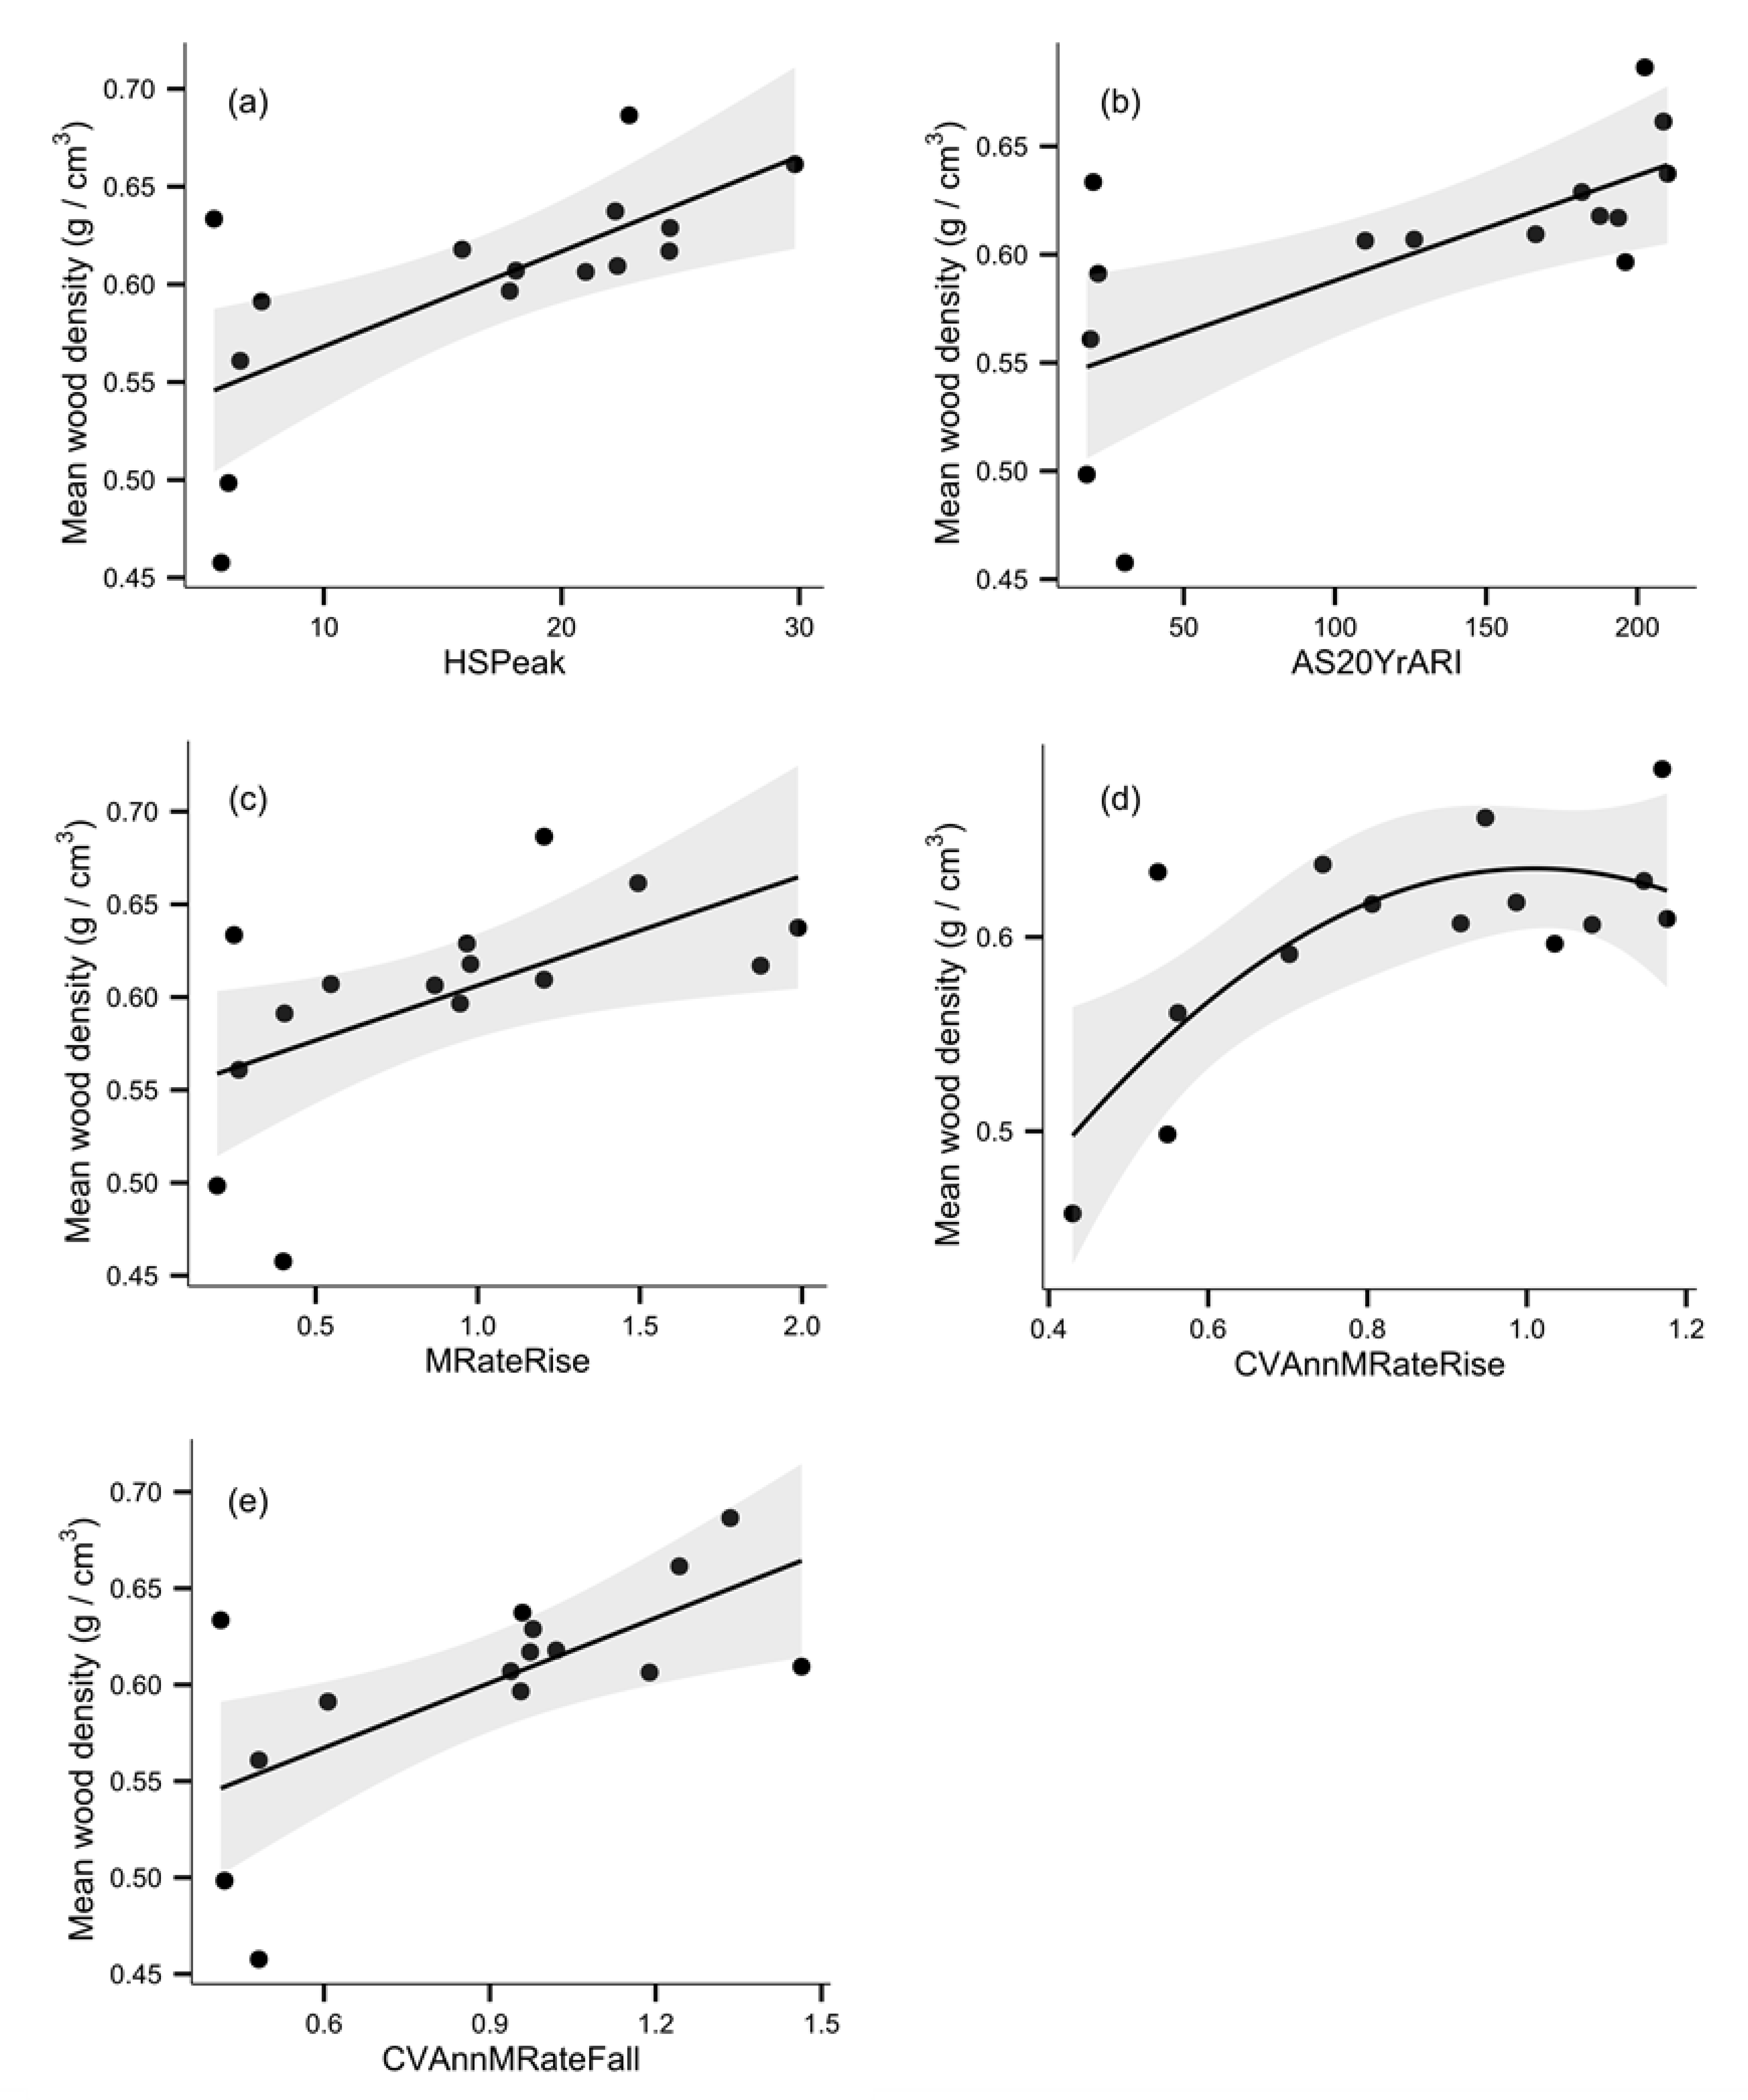
\includegraphics[width=\textwidth,keepaspectratio=true]{Ch2Fig2.png} % figures can be in pdf, png, jpeg or eps format
\caption[Relationships between wood density and flood magnitude and frequency.]{\small{Relationships between community weighted mean wood density and hydrological metrics describing a.) mean high flow magnitude (HSPeak), b.) magnitude of the 20 year average return interval flood (AS20YrARI), c.) mean rate of flow rise (MRateRise), d.) interannual variability in flood rise rates (CVAnnMRateRise), e.) interannual variability in flood fall rates (CVAnnMRateFall). Fitted lines depict ordinary least squares regression models. d. is a quadratic fit, all other models are linear fits. Shaded areas depict the smoothed 95 \% confidence interval around the regression model.}}
\label{fig:Ch2_F2} % label for cross-referencing
\end{center}
\end{figure}   
\clearpage

We found denser woody tissues were increasingly favoured as baseflow index decreased (Fig. \ref{fig:Ch2_F3}a). Wood density increased as patterns of average flow conditions became a) less uniformly distributed across seasons (Fig. \ref{fig:Ch2_F3}b), and b) less uniformly distributed year to year (Fig. \ref{fig:Ch2_F3}c). Thus mean wood density is maximised when average flow patterns are highly seasonal, but the season with which they are associated is not consistent throughout the record. A similar relationship was observed for inter-seasonal (Fig. \ref{fig:Ch2_F3}d) but not inter-annual uniformity of minimum flows. In other words, wood density was highest where minimum flows were not associated with any particular season.  Mean wood density also increased with increasing interannual variability in baseflow index (Fig. \ref{fig:Ch2_F3}e), pointing to a strong effect from years in which baseflow deviated from the mean. Wood density also decreased with mean low spell flow (Fig. 3f), and with the mean 7-day minimum flow (Fig. \ref{fig:Ch2_F3}g). For both metrics, higher values indicate wetter minimum flow conditions. Mean wood density also increased with low flow frequency (Fig. 3h). Metrics of low flow duration were not significantly associated with wood density.

No significant pattern of spatial autocorrelation was detected within values of CWM (P = 0.228). 
\begin{figure}[ht]
\begin{center}
\includegraphics[height=0.85\textheight,keepaspectratio=true]{Ch2Fig3.png} % figures can be in pdf, png, jpeg or eps format
\caption[Relationships between wood density and variability in water availability]{\small{Relationships between community weighted mean wood density and hydrological metrics describing a.) baseflow index (BFI), b.) contingency of monthly mean daily flow (M\_MDFM), c.) constancy of monthly mean daily flow (C\_MDFM), d.) constancy of monthly minimum daily flow (C\_MinM), e.) interannual variability in baseflow index (CVAnnBFI), f.) mean low flow magnitude (LSPeak), g.) mean flow during driest week of the year (MA.7days.MinMean), h.) annual frequency of low flows (MDFAnnLSNum). c. � e. are quadratic fits, all other models are linear fits. Shaded areas depict the 95 \% confidence interval around the regression model}}
\label{fig:Ch2_F3} % label for cross-referencing
\end{center}
\end{figure}   
\clearpage

\subsection{What are the principal components of variation in hydrological conditions that explain variation in wood density?}
Hydrological metrics that significantly explained site mean wood density were highly correlated in our dataset. Principal Components Analysis (PCA) identified one dominant axis within these metrics, representing 80.3 \% of variation (Fig. \ref{fig:Ch2_F4}). The remaining variation was split between several minor axes; PCA2 represented 6.3 \% of variation and the remaining axes each represented less than 3 \% of variation.

PC1 represents a gradient of environmental harshness that integrates baseflow characteristics, seasonality and flooding intensity. Metrics which are maximised under conditions of weak seasonality, high predictability and low variability of water availability were loaded towards the positive end of the PC1 axis, while metrics that are maximised under conditions of high interannual baseflow variability and high intensity flooding were loaded towards the negative end. Stable winter baseflow rivers exhibited lower site mean wood density, and were clustered at the �mild� positive end of the PC1 gradient. Unpredictable baseflow and unpredictable intermittent rivers overlapped across PC1 and were located distally towards the �harsh� negative end, and were associated with higher site mean wood density. The results of the PCA analysis illustrated that variation in wood density is largely described by a single axis of variation from low to high variability in flow.

\begin{figure}[h]
\begin{center}
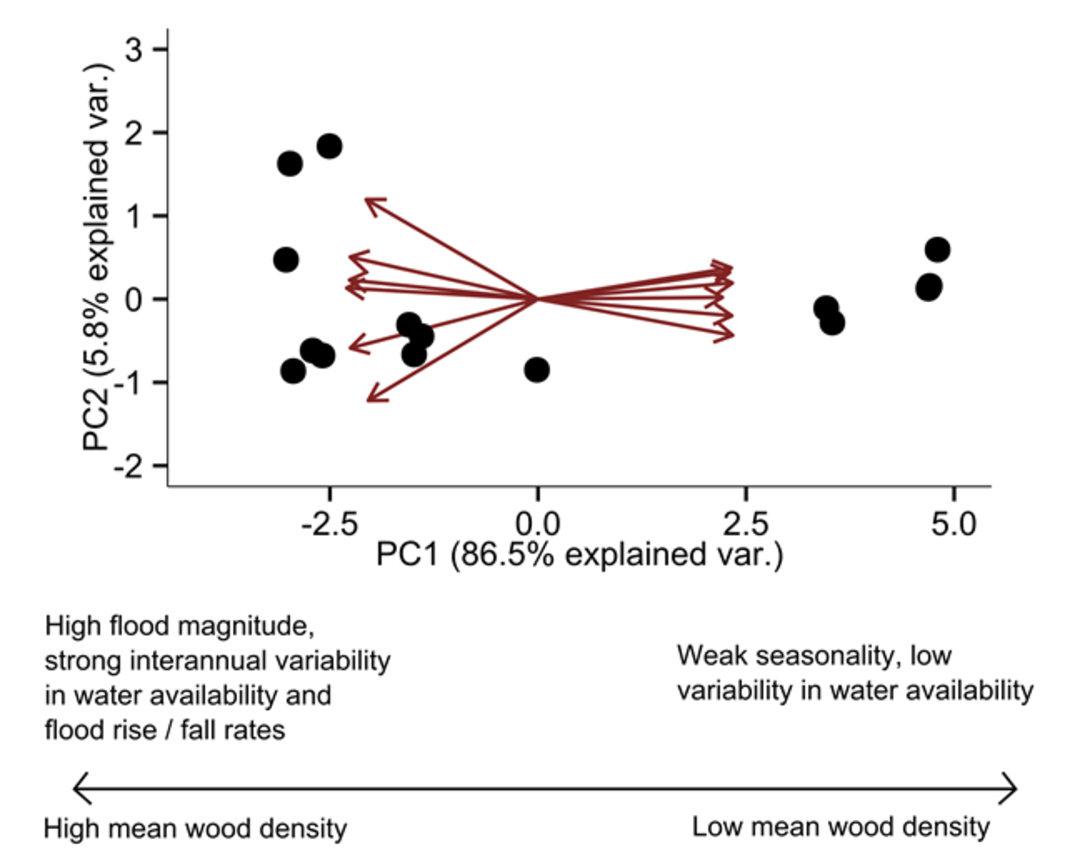
\includegraphics[width=12cm]{Ch2PCAbiplot.pdf} % figures can be in pdf, png, jpeg or eps format
\caption[PCA biplot of sites according to significant hydrological relationships with wood density.]{\small{Biplot of sites ordinated across the first two principal components as determined from Principal Components Analysis of hydrological metrics displaying significant relationships with mean wood density across 15 sites in south eastern Australia. Points represent individual sites. PC1 explains 80.3 \% of the variation in hydrology among the sites and represents a gradient of harshness of environmental conditions.}}
\label{fig:Ch2_F4} % label for cross-referencing
\end{center}
\end{figure}   

\subsection{Is there a relationship between hydrological disturbance and within-community dispersion of wood density?}
No individual metrics describing hydrological disturbance showed significant relationships with CWV following p-value adjustment. The relationship between the PC1 axis and CWV in wood density could be significantly explained by a quadratic model, however (R2 = 0.450, P = 0.037) (Fig. \ref{fig:Ch2_F5}). The fitted curve shows a peak in CWV at intermediate values of PC1, which correspond to intermediate values of hydrological disturbance and variability. No significant pattern of spatial autocorrelation was detected within values of CWV (P = 0.786).

\begin{figure}[ht]
\begin{center}
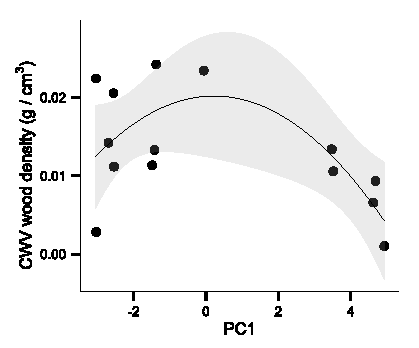
\includegraphics[width=9cm]{Ch2CWV.pdf} % figures can be in pdf, png, jpeg or eps format
\caption[Unimodal relationship between wood density CWV and PC1.]{\small{Quadratic relationship between community weighted variance in wood density and site scores for the first principal coordinate (PC1) of a Principal Components Analysis of hydrological metrics displaying significant relationships with mean wood density (see Fig. 4), (R2 = 0.450, P = 0.037). Variance peaks at intermediate values of hydrological disturbance, as described by the PC1 axis. Shaded areas depict the 95 \% confidence interval around the regression model.}}
\label{fig:Ch2_F5} % label for cross-referencing
\end{center}
\end{figure}   
\

\section{Discussion}
We sought to understand how hydrology might influence wood density, a key plant functional trait. We asked whether mean wood density could be explained by the degree of flooding disturbance or hydrological unpredictability in the riparian zone, and whether dispersion of wood density peaks in intermediately disturbed communities. To summarise, we found evidence that mean riparian wood density is positively related to flood magnitude and flow rise and fall rates, as well as to unpredictability in flow conditions over daily, seasonal and annual timescales. We also found evidence for divergence in wood density strategy at intermediate levels of disturbance.  While wood density is a complex trait that integrates trade-offs between multiple selection pressures, we believe the strong relationships between mean wood density and hydrology demonstrated here are evidence that hydrological conditions powerfully influence plant ecological strategy in the riparian environment. 

Strong relationships with measures of interannual variability point to years in which the environment was extreme as favourable towards high wood density. Several relationships were described best by quadratic models, indicating a maximum above which variation in hydrology ceases to be associated with changes in mean wood density. Predictable hydrologies and weak flooding disturbance intensity were associated with a greater range of mean wood density values. This variability may be driven by other environmental factors, which become less influential as hydrological forcing increases.  We also found that for \textit{Casuarina cunninghamiana}, a common riparian species in SE Australia, intraspecific variation in wood density responded strongly to hydrology (see Appendix 1, Fig. \ref{fig:Ch2sup_F1}).

Specific aspects of high flow hydrology drove variation in wood density. Mean wood density was not correlated with the frequency of high flow spells, which individually may not correspond to significant disturbance events, depending on the hydrological characteristics of the given river. Rather, it was the actual magnitude of flow during high flow periods that was important. High rates of flow rise and fall, which may associated with entrainment of large debris into the flood channel and subsequent bank deposition \citep{Cadol2010}, were also associated with high community wood density. Interannual variability in rate of flow rise was a substantially stronger predictor of wood density than the mean value, suggesting a greater influence of flow rise rates in extreme years than the general mean. A pattern is apparent then, in which mean wood density in riparian communities is driven by powerful but relatively rare flow events (e.g. 10 to 20 year average return interval flood). Such floods are likely to be large enough to influence demographics, but not necessarily catastrophic (i.e. presenting no opportunity for survival). The abundance of high wood density strategies in these environments indicates that infrequent but high-stakes events may be a greater selective pressure in riparian plant communities than average conditions. For densely wooded species, persistence may be more influential on population dynamics than individual growth rates or fecundity \citep{Adler2014}. We therefore suggest that a �brick house� ecological strategy is favoured in riparian environments that experience intense flooding. This suggestion concurs with findings that trees on windy slopes tend to overcompensate for mechanical stress, with investment in defences increasing cumulatively in response to stress events \citep{telewski1995wind, Cohen1999}. This cumulative effect may be important for long-lived woody species which experience multiple high magnitude floods during their lifetimes.
 
We can extend the observation about the influence of intense �pulse� flow events on wood density: plants living in environments where flow occurs unpredictably and largely within specific events, rather than being evenly distributed throughout time, are likely to experience more intense pulses of water stress (i.e. low soil moisture). High wood density may be symptomatic of wood anatomy strategies that allow plants to tolerate water stress \citep{Hacke2001, Jacobsen2005, Jacobsen2007}. Numerous studies have discussed the role of various anatomical components of woody tissue in stabilising xylem against cavitation when plants are under severe water stress, but the exact role that woody fibres play in stabilising xylem vessels appears to be inconsistent \citep{Martinez-Cabrera2009}. Overall, resistance against cavitation emerges from complex interactions between wood anatomical traits \citep{Lens2011, Zieminska2013} and$/$or aboveground biomass production traits, both of which are tangentially related to wood density. With the exception of ephemeral dryland rivers, riparian environments tend not to be severely water limited, so specifically constructing woody tissue to deal with constant water stress may not be advantageous. For plants that are habituated to plentiful soil moisture, however, having no backup strategy for surviving drought conditions may be risky \citep{Horton2013}.

A more compelling rationale for our findings is that riparian woody plants are again overcompensating for the possibility of uncommon but intense stress events. In the absence of predictable cues about timing of watering flows, conservative resource-use phenotypes such as higher wood density would be favoured \citep{Valladares2007}. Environmental unpredictability may act as a modifier which shifts ecological strategy in favour of conservative resource use (for which wood density acts as a proxy, in this case). We can observe this effect in intraspecific variation (see Appendix 1, Fig. 1) in wood density for the rheophytic (i.e. confined to frequently flooded substrates) species \textit{C. cunninghamiana}: interannual variability in baseflow index, contingency of monthly minimum daily flow (M\_MinM) and contingency of monthly mean daily flow (M\_MDFM) describe interannual variability in water availability and all show strong relationships with intraspecific variation in \textit{C. cunninghamiana} wood density. Traits associated with conservative resource use and better recovery following periods of stress may actually confer as much or greater fitness than traits associated with coping with the stress itself \citep{Gutschick2003}.
  
Conservative resource use and heavy investment in structural strength fit within the �resister� category of riparian plant strategies described by Naiman \& Decamps' (1997) classification of riparian plant life history strategies. �Invader� strategies with which species avoid harsh hydrological conditions by achieving sexual maturity as fast as possible are also common to the riparian environment \citep{Naiman1997, Woolfrey2001}. For pioneer species employing a fast relative growth rate, low wood density ecological strategy would be benefited by repeated setbacks to early successional conditions \citep{Westoby1998}. Co-existence at intermediate disturbance intensities of a broad spectrum of strategies between �invading� and �resisting� may be responsible for the observed peak in wood density CWV, but this suggestion is difficult to substantiate using our dataset, as only a few sites were present in the middle range of the PC1 axis.
 
Under our argument, where hardy rheophytic species use high wood density ecological strategies to cope with powerful floods and unpredictable watering regimes, we would expect species such as \textit{Casuarina cunninghamiana} (Casuarinaceae) and \textit{Tristaniopsis laurina} (Myrtaceae) (two of the most common riparian species in our study region) to have the highest wood density in our dataset. However both species exhibited highly variable trait values, ranging approximately between the median value and the 75th percentile. As with \textit{C. cunninghamiana}, \textit{T. laurina} is a light-demanding coloniser of within- and near-channel landforms \citep{Webb2002}. By establishing in close proximity to the channel, seedlings of these species must balance the risks of flooding with the advantages of growth unencumbered by competition for light or space. Maintaining a high relative growth rate, at least until the trees are physically large enough to endure flooding, allows these species to quickly fill space and build photosynthetic tissue (i.e. invading) \citep{Melick1990}. If parallels with tropical rainforest species hold \citep{King2006, Kraft2008, Poorter2008, Poorter2010, Wright2010}, this strategy will not be conducive to setting down dense wood (i.e. resisting). In addition to morphological adaptations in \textit{T. laurina} such as multi-stemmedness, narrow leaves and growth streamlined against the direction of flow \citep{steenis1981rheophytes, Webb2002}, the trade-off between flood resistance and rapid resource acquisition and growth during establishment serves to explain why the optimal wood density for rheophytic species might occupy a central position along the axis of wood density. Nonetheless, the wide plasticity in wood density shown by \textit{C. cunninghamiana} and \textit{T. laurina} suggests that intraspecific variation contributes to the species� capacity to track hydrological gradients. Thus intraspecific variation in these species influences community mean wood density despite their relatively moderate species-specific mean wood density.
 
Notably, it is the tall, facultative riparian species from rainforest sites that had the highest wood density in our dataset. Lacking the morphological adaptations required to thrive directly along the channel edge, these species may rely solely on generating mechanically strong stems to withstand flooding. High wood density species tended to occur further up the bank, so would be subject to only the more intense flooding events (and least moisture availability). Since succession typically advances with elevation above the channel edge \citep{Tabacchi1998}, this observation agrees with previous work showing increasing wood density along a successional gradient \citep{Falster2005}. Further parallels in the existing wood density literature are also evident here, where high wood density individuals were much less likely to experience major wind damage following a cyclone \citep{Curran2008}.

The gradient identified by principal components analysis integrates predictability of water availability, seasonality and flood intensity into a single axis of hydrological variation. It is not possible to tease out individual drivers of variation in mean wood density, as the conditions associated with both environmental unpredictability and mechanical disturbance act in unison to drive community wood density towards higher mean values.
 
Community weighted variance in wood density showed a quadratic distribution across this gradient of �hydrological harshness�. Previous work has described a negative relationship between community-level variance in wood density and abiotic stress (using high latitude and elevation as proxies for stressful environments) \citep{Swenson2007}. Rather than constricting trait values, intermediate levels of pulsed fluvial disturbance may promote trait diversity by retarding competitive exclusion \citep{Huston1979, Naiman1997}, whilst simultaneously generating structurally heterogeneous habitat \citep{Corenblit2007}. While the fit of our model is statistically significant, the paucity of values through the middle range of the PC1 axis gives rise to error around the peak of the fitted curve; interpretation of this result therefore necessitates some caution.
 
Damming and water extraction, and changing climatic conditions are altering hydrology globally \citep{Nilsson2000, stocker2013climate}. Artificial flow modification by damming and water extraction reduces overall flow volume and the magnitude and frequency of high flow events, while increasing flow predictability, altering seasonality and limiting channel-floodplain connectivity \citep{Maheshwari1995, Graf2006}. In these altered conditions, terrestrial species with softer wood and faster growth rates may encroach on what was once the province of rheophytic assemblages adapted to flooding and less predictable hydrological conditions. The converse of this situation is presented by predictions of future climatic conditions: in Australia, warming of 0.4 - 0.7  \textsuperscript{o}C has occurred since 1950 \citep{Hennessy2007}, associated with a reduction in rainfall across southern and eastern regions of the continent \citep{Smith2004}, and an increase in intensity and frequency of droughts \citep{Hennessy2008}. Extreme rainfall events are predicted to become more prevalent, even in areas where the trend is towards mean reductions in annual or seasonal rainfall \citep{Chiew2009}. River discharge in Australia is known to be particularly sensitive to the El Nino-Southern Oscillation (ENSO)  phenomenon that is an integral driver of the continent's climate patterns \citep{Nicholls1989, Ward2010}. Projected increases in climatic variability \citep{Hennessy2008} may therefore overlay the already strong natural variability induced by ENSO to produce significant alterations to streamflow. Under such conditions, near-channel abundance of opportunistic terrestrial species (with their broad diversity of wood density strategies) may decline in favour of rheophyte-dominated assemblages whose ecological strategies are optimized to harsh hydrological conditions.  If changes in spatial extent of climate zones can be related to changes in runoff - a complicated but progressing area of research in hydroclimatology \citep{Peel2011} - functional approaches to ecohydrology can give insight into likely changes in riparian plant assemblages and associated changes in ecosystem function.

\section*{Conclusion}
Our study emphasises the importance of hydrological conditions, particularly disturbance and environmental unpredictability, as determinants of ecological strategy in riparian plant communities. These relationships may be generalisable to diverse biomes, given the strong constraints imposed by flooding and fluctuating water availability on woody plant ecological strategies in many riparian environments.  The marked influence of rare, high intensity floods on wood density is likely to have significant ecological consequences for riparian plant communities in a south-east Australian context, and potentially in other regions where increasing climatic variability and frequency of extreme events are hallmarks of climate change predictions.

\section*{Acknowledgements}
Tanja Lenz gave invaluable advice and support throughout the project. Saskia Grootemaat, Ashley Vey, Urvashi Lallu, Julia Atkinson, Sally Lawson and Anthony Manea gave their time and inspiration in the field. We also wish to thank the officers of the New South Wales Parks and Wildlife Service and Parks Victoria who provided logistical advice and support, and the landowners who were so kind as to let us work and stay on their properties. Thanks also to Alan Baldry for his help in the herbarium, and to the PIREL group at Macquarie University for their support. Finally, we would like to thank Stephen Bonser and two anonymous reviewers for their knowledge and insight.

\section*{Data availability}
Data are available through DataDryad, doi:10.5061/dryad.72h45 \citep{Lawson2015}.
\clearpage


%%%%% REFERENCES % this is in a new chapter due to the memoir format
\renewcommand\bibname{{References}} 
\begin{small}
\bibliographystyle{apalike}
\bibliography{library.bib}
\end{small}








